% $Id: board1.tex 9464 2021-10-14 16:51:12Z mskala $

%
% MSK 014 Board 1 build instructions
% Copyright (C) 2022  Matthew Skala
%
% This program is free software: you can redistribute it and/or modify
% it under the terms of the GNU General Public License as published by
% the Free Software Foundation, version 3.
%
% This program is distributed in the hope that it will be useful,
% but WITHOUT ANY WARRANTY; without even the implied warranty of
% MERCHANTABILITY or FITNESS FOR A PARTICULAR PURPOSE.  See the
% GNU General Public License for more details.
%
% You should have received a copy of the GNU General Public License
% along with this program.  If not, see <http://www.gnu.org/licenses/>.
%
% Matthew Skala
% https://northcoastsynthesis.com/
% mskala@northcoastsynthesis.com
%


\chapter{Building Board 1}\label{ch:board1}

Board~1 has components on both sides, and for best results, it is important
to install them in the right order.  Build Board~2 first, and see the
general comments in the Board~2 chapter about how to approach the task.

\section{Preliminaries}

Count out the right number of everything according to the bill of materials. 
There is an abbreviated BOM for the items needed in this chapter (including
the connection to Board~2 and final assembly of the module) in
Table~\ref{tab:b1bom}.

\nopagebreak
\noindent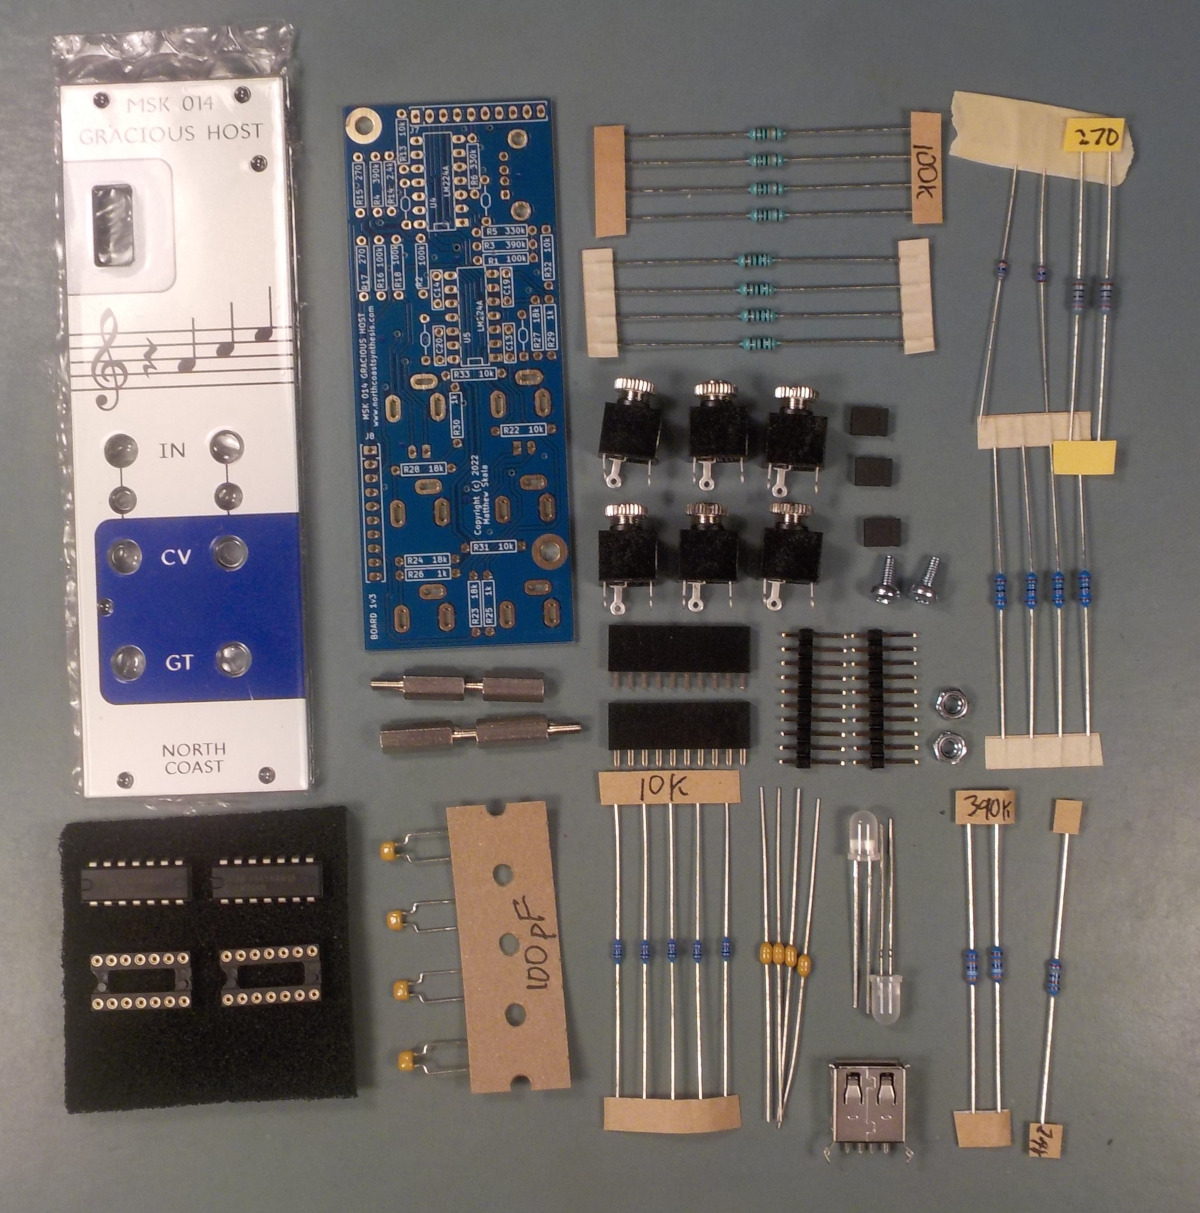
\includegraphics[width=\linewidth]{board1-parts.jpg}

\begin{table*}
{\centering
\fbox{This table is not a substitute for the text instructions.}
\vspace{\baselineskip}

\begin{tabular}{rp{1.3in}cp{3in}}
  \textbf{Qty} & \textbf{Ref} & \textbf{Value/Part No.} & \\ \hline
\input{bomdata-1.tex}
\end{tabular}\par}
\caption{Bill of Materials for Board~1.
Also needed:
the PCB itself, the aluminum front panel,
the assembled Board~2, three configuration jumpers,
and panel-to-rack mounting hardware.}\label{tab:b1bom}
\end{table*}

\section{Decoupling capacitors}

The four axial ceramic 0.1$\mu$F decoupling capacitors C1, C2, C17, and C18
are shown on the board by a special symbol without their reference
designators.

\nopagebreak
\noindent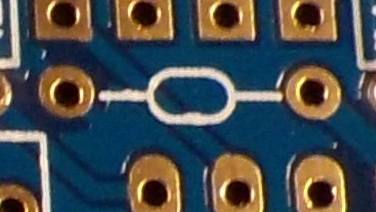
\includegraphics[width=\linewidth]{decoup-symbol.jpg}

Install these four capacitors where the symbol appears.  They are not
polarized and may be installed in either orientation.  These capacitors act
as filters for the power supplies to the op amp chips, protecting them from
high-frequency crosstalk.

\nopagebreak
\noindent\includegraphics[width=\linewidth]{{cap-0.1u1}.jpg}

\section{Fixed resistors}

Resistors are never polarized.  I like to install mine in a consistent
direction for cosmetic reasons, but this is electrically unnecessary.  In
this module, the fixed resistors are metal film 1\%\ type.  They usually
have blue bodies and four colour bands designating the value, plus a fifth
band for the tolerance.  The tolerance band is brown for 1\%, but note that
we may occasionally ship better-tolerance resistors in the kits than the
specifications require, if we are able to source them at a good price. 
Accordingly, I mention only the four value band colours for this type of
resistor; if you are using resistors with other codes, you are responsible
for knowing them.  Note that colour codes on metal film 1\% resistors are
often ambiguous (reading from one end or the other end may give two
different values, both plausible) and some of the colours are hard to
distinguish anyway.  If in doubt, always measure with an ohmmeter before
soldering the resistor in place.

Install the two 270$\Omega$ (red-violet-black-black) resistors R15 and R17. 
These set the current level for the front-panel LED driver circuits.

\nopagebreak
\noindent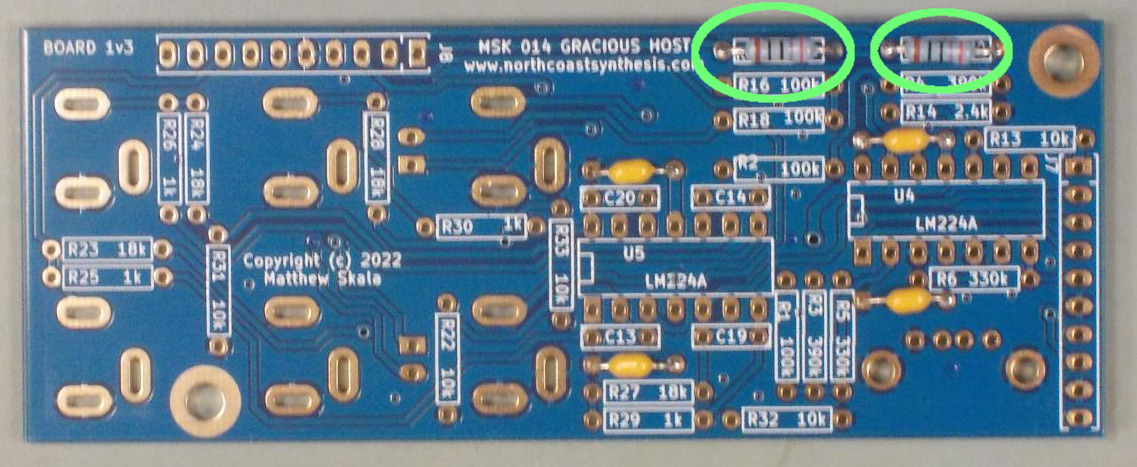
\includegraphics[width=\linewidth]{res-270.jpg}

Install the four 1k$\Omega$ (brown-black-black-brown) resistors R25, R26,
R29 and R30.  These are current-limiting resistors to protect the output
drivers, and other modules, in case of short circuits or bad patching on the
output jacks.

\nopagebreak
\noindent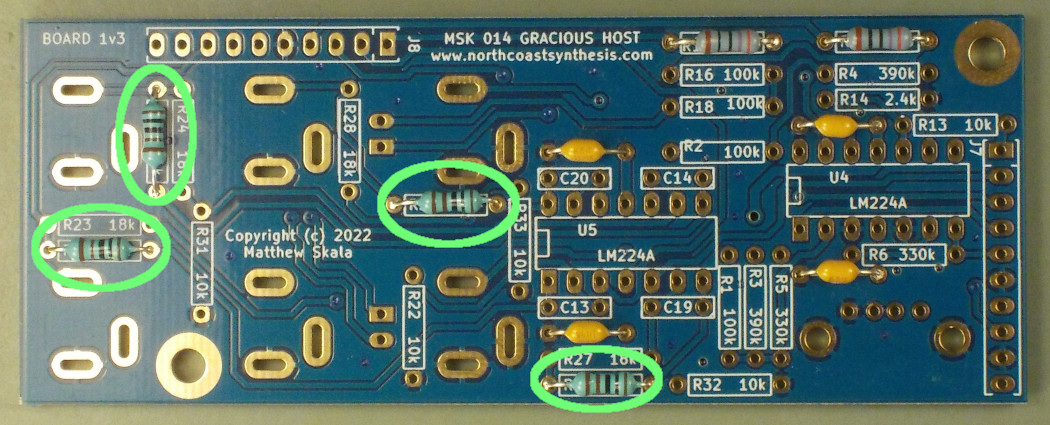
\includegraphics[width=\linewidth]{res-1k.jpg}

Install the single 2.4k$\Omega$ (red-yellow-black-brown) resistor R14.
This is part of a voltage divider (with R13) that sets the relative balance
of current levels between the red and green LED colours, to make them
roughly equally bright given their different current sensitivity levels.

\nopagebreak
\noindent\includegraphics[width=\linewidth]{{res-2.4k}.jpg}

Install the five 10k$\Omega$ (brown-black-black-red) resistors R13, R22, and
R31 to R33.  R13 is part of the voltage
divider with R14, and the other four are used for setting the gain of the
output driver amplifiers.

\nopagebreak
\noindent\includegraphics[width=\linewidth]{{res-10k1}.jpg}

Install the four 18k$\Omega$ (brown-grey-black-red) resistors R23, R24, R27,
and R28.  These are feedback resistors for the output driver amplifiers,
setting the voltage gain (to 2.8 non-inverting) in conjunction with the
10k$\Omega$ resistors.

\nopagebreak
\noindent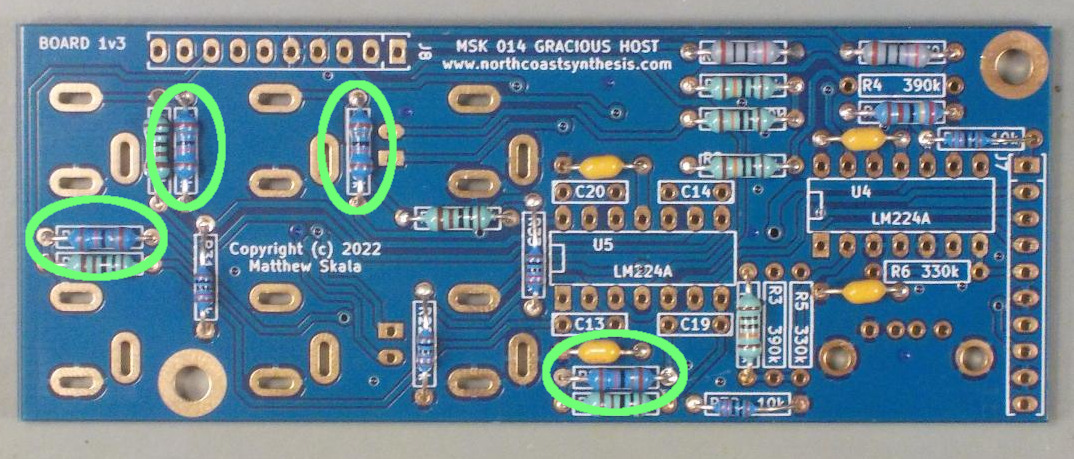
\includegraphics[width=\linewidth]{res-18k.jpg}

Install the four 100k$\Omega$ (brown-black-black-orange) resistors R1, R2,
R16, and R18.  The first two of these, R1 and R2, are input resistors that
set the input impedance for the CV input jacks.  The others, R16 and R18,
set the default input voltage of the LED drivers when the microcontroller
disconnects, so that an ``LED off'' command will correspond to little or no
current through the LEDs.

\nopagebreak
\noindent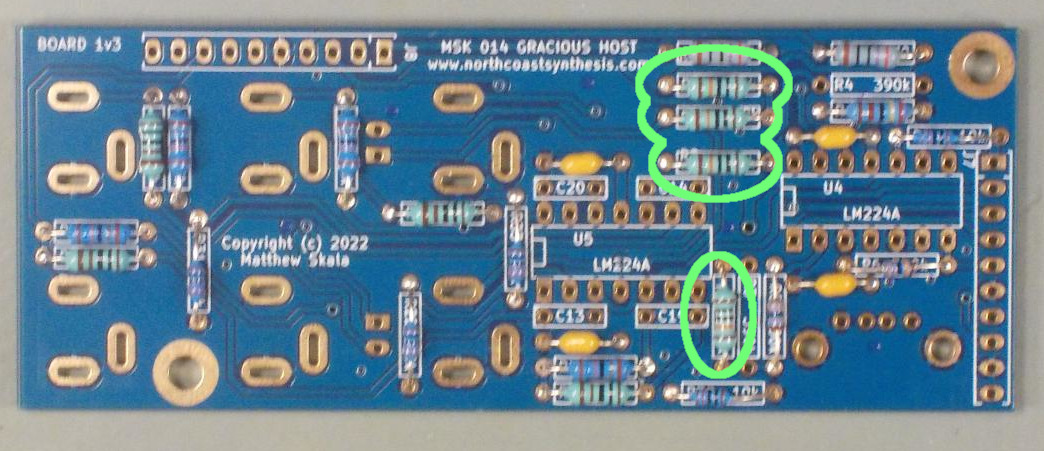
\includegraphics[width=\linewidth]{res-100k.jpg}

Install the two 330k$\Omega$ (orange-orange-black-orange) resistors R5 and
R6.  These are feedback resistors for the input buffer op amps.

\nopagebreak
\noindent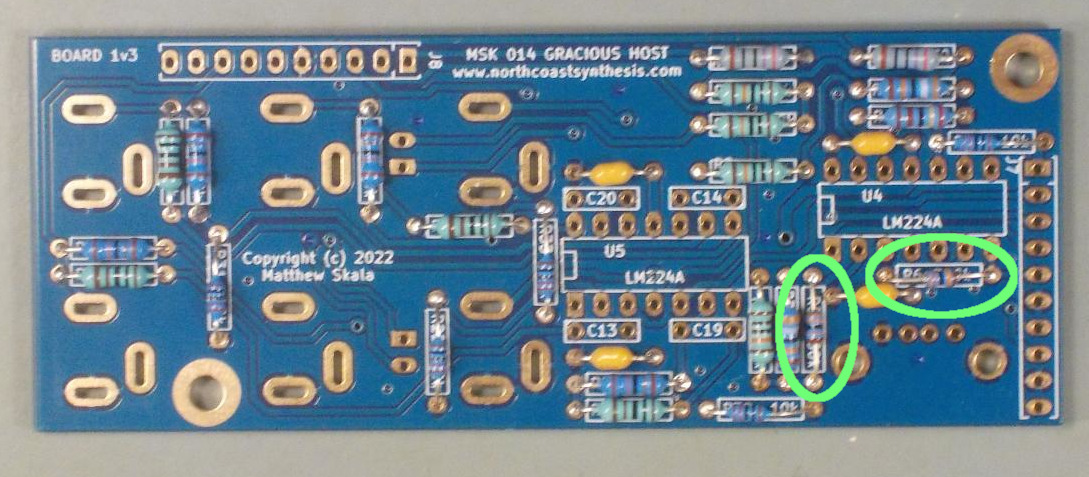
\includegraphics[width=\linewidth]{res-330k.jpg}

Install the two 390k$\Omega$ (orange-white-black-orange) resistors R3 and
R4.  These apply an offset to the input buffers, with the effect of shifting
the op amp's clipping range to cover just beyond the intended 0V--5V input
range.

\nopagebreak
\noindent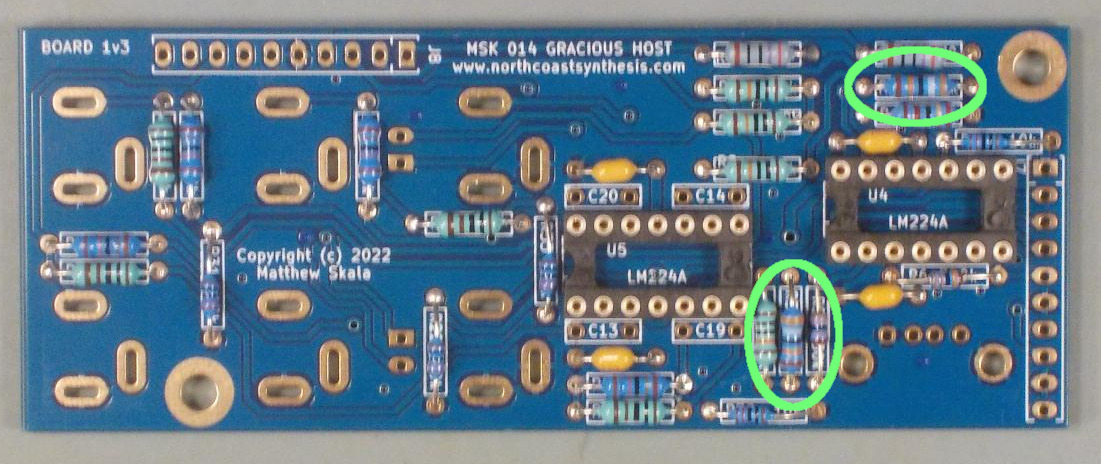
\includegraphics[width=\linewidth]{res-390k.jpg}

\section{DIP sockets}

Install the 14-pin DIP sockets for the LM224 quad operational
amplifier (op amp) chips U4 and U5.  The boards or chips may be labelled
LM224A, with or without some other alphabetic suffix; the plain and -A versions
have slightly different specifications but both will work in this circuit.
Of the eight amplifier units on these
two chips, two are used as LED drivers, and the rest are assigned one each
to the front panel patching jacks:  two input buffers and four output
drivers.

DIP sockets
themselves do not care which direction you install them, but it is
critically important that the chip installed in the socket should be
installed in the right direction.  To help with that, the socket will
probably be marked with notches at one end (indicating the end where Pin~1
and Pin~14 are located) and you should install the socket so that the
notched end matches the notch shown on the PCB silkscreen.  The solder pad
for Pin~1 is also distinguished by being rectangular instead of rounded.

Installing DIP sockets without having them tilted at a funny angle can be
tricky.  I recommend inserting the socket in the board, taping it in place
on the component side with vinyl electrical tape or sticking it there with a
small blob of putty at each end, then soldering one pin on
one corner and checking that the socket is snug against the board before
soldering the other pins.  That way, if you accidentally solder the first
pin with the socket tilted, it will be easier to correct (only one pin to
desolder instead of all of them).

\nopagebreak
\noindent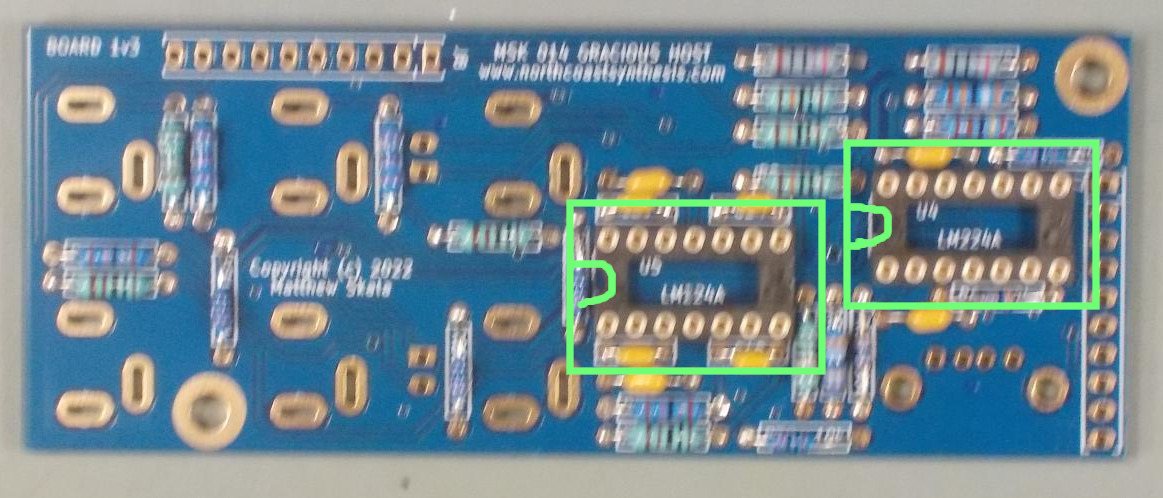
\includegraphics[width=\linewidth]{dip14.jpg}

\section{Compensation capacitors}

Install the 100pF radial ceramic capacitors C13, C14, C19, and C20.  These
are meant to ensure stability of the output drivers (one each).  The
capacitors will probably be marked ``101,'' for 1 0 followed by one more 0,
number of picofarads.  They are not polarized and may be installed in either
direction.

\nopagebreak
\noindent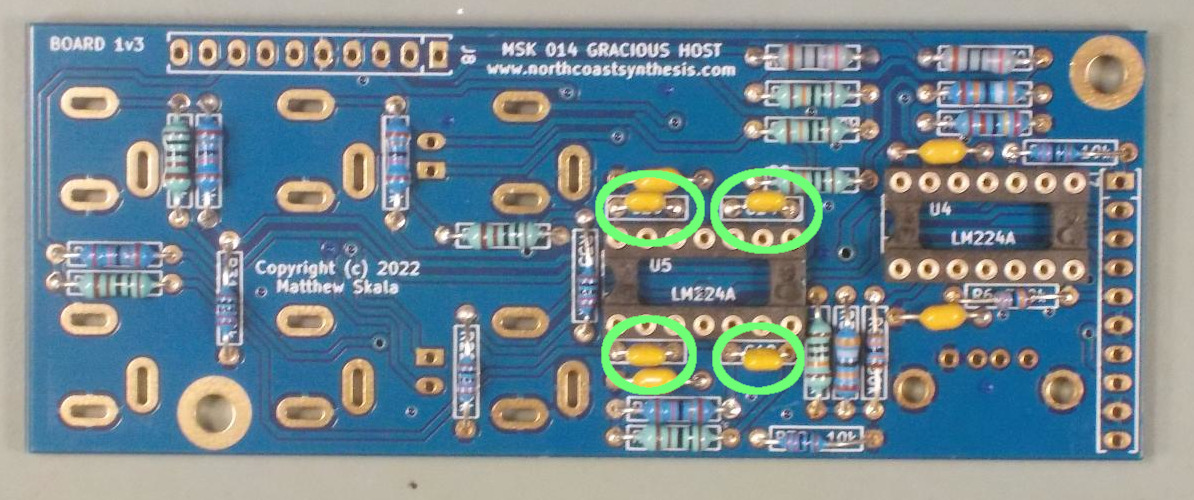
\includegraphics[width=\linewidth]{cap-100p.jpg}

\section{Board to board connectors}

Fasten the two 13mm standoffs on the back of Board~1; that is the side
opposite the components already installed.  Attach them with the two 11mm
standoffs.  The male ends of the 13mm standoffs should pass through the
mounting holes in the board and mate with the female ends of the 11mm
standoffs on the front or component side of the board.

Mate the 10$\times$1 header connectors J7 and P2 and place them (do not
solder yet) in the J7 footprint on Board~1 with the legs of the female
connector J7 going through the board.  Similarly, mate J8 and P3 and place
them (do not solder yet) in the J8 footprint on Board~1.

\nopagebreak
\noindent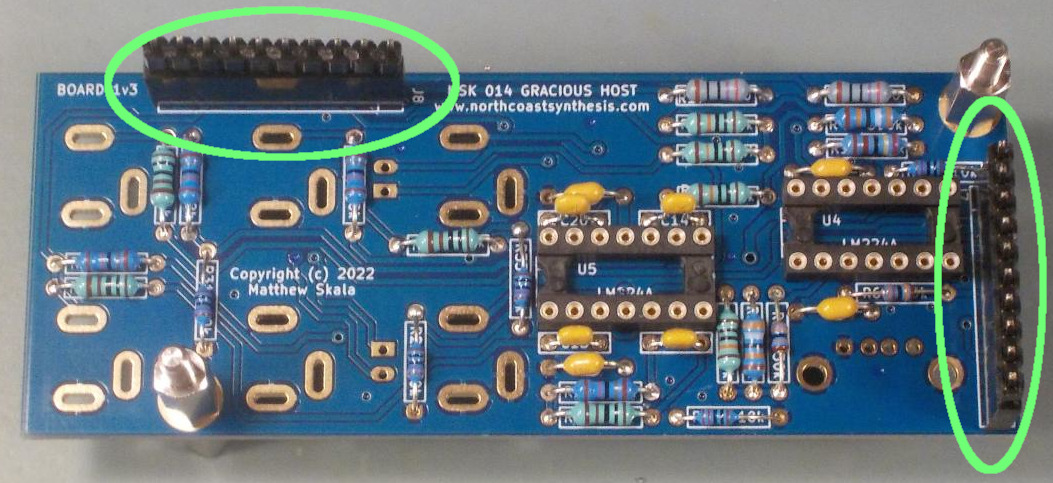
\includegraphics[width=\linewidth]{board-to-board.jpg}

Place your completed Board~2 from the previous chapter on top of the
assembly, component side up with the legs of P2 and P3 going through the
corresponding footprints, and fasten the board to the 11mm standoffs with
the two hex nuts.  The resulting temporary assembly should be as shown in
the photo.

\nopagebreak
\noindent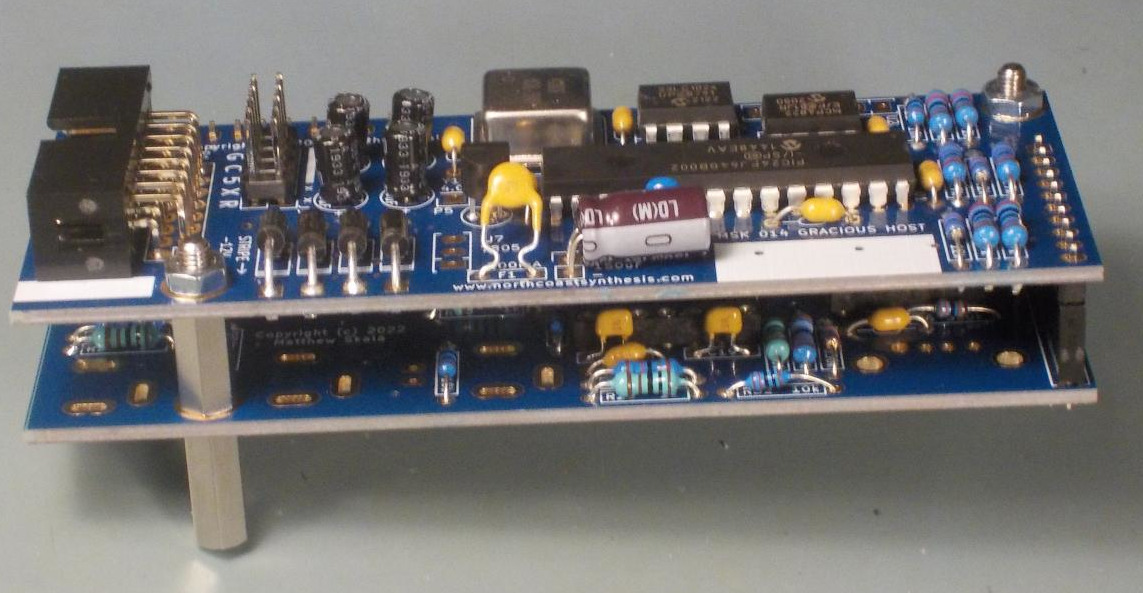
\includegraphics[width=\linewidth]{temp-assy.jpg}

Solder J7, J8, P2, and P3 in place on the two boards.  Then remove Board~2
and the hex nuts holding it in place, but keep the standoffs that go through
the holes in Board~1.

\section{Panel components}

Flip Board~1 over; you will now be installing the components that go between
it and the panel.  The pieces fit together in a straightforward way, but
see the exploded assembly diagram on page~\pageref{fig:exploded} if
further clarification is needed.

Place (do not solder yet) the six phone jack sockets J1 through J6 in
their footprints.  These are for patching signals to and from other modules. 
These components should only be able to fit into the board in one way.

\nopagebreak
\noindent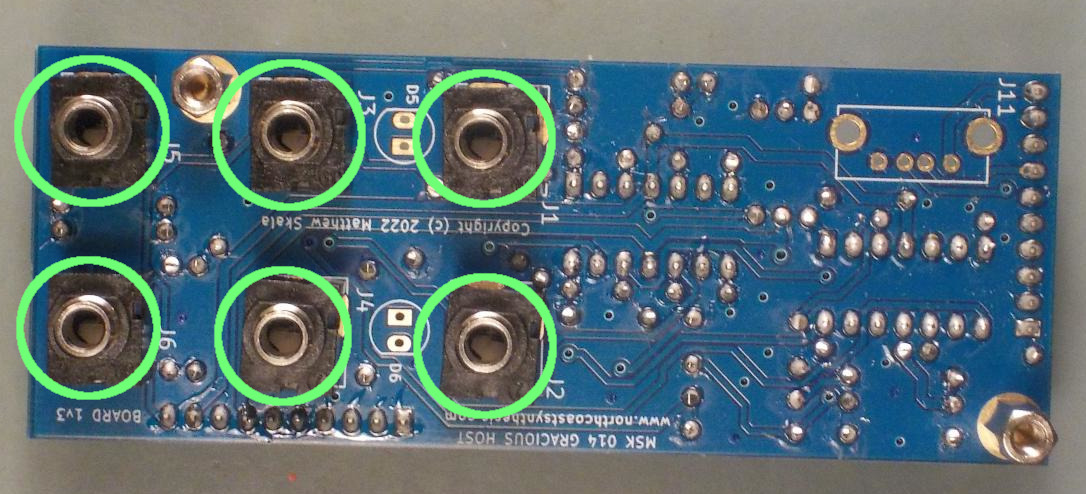
\includegraphics[width=\linewidth]{jack.jpg}

Place (do not solder yet) the two bi-colour LEDs D5 and D6 in their
footprints.
Single LEDs are polarized and can be destroyed by reverse
voltage.  These ones here are special bi-colour devices with two separate
LEDs in each package.  The internal connection is such that each one
protects the other from reverse voltage; so if connected backwards, they
will not be destroyed, but the intended green and red colours will be
swapped.  Each LED lens has one flat side, and one leg shorter than the
other on that side.  The short leg is Pin~1.  Its proper place on the board
is marked by a circle with a flattened side matching the direction of the
flattened side on the LED lens, and an oval solder pad.  The other leg
(Pin~2, long, farther from the flat side) goes into the rectangular solder
pad.  Be sure both LEDs are placed right way around according to these
clues.

\nopagebreak
\noindent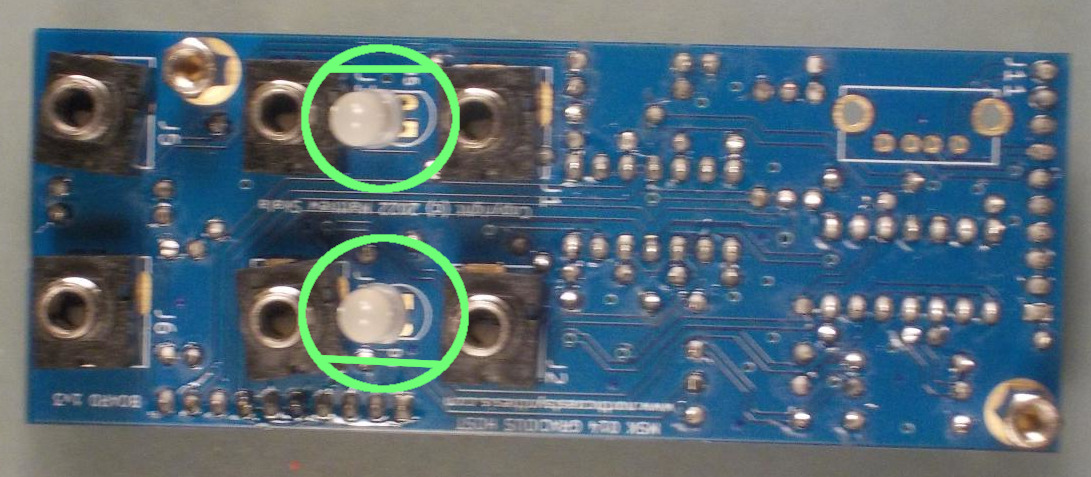
\includegraphics[width=\linewidth]{led.jpg}

Place (do not solder yet) the USB~A connector J11 in its footprint on the
board.  There should be only one orientation in which it will fit.  The tabs
on the back of the connector will snap into the mounting holes on the board,
holding the connector in place; but you may need to adjust its angle
slightly, especially in the next step when it fits into the panel.

\nopagebreak
\noindent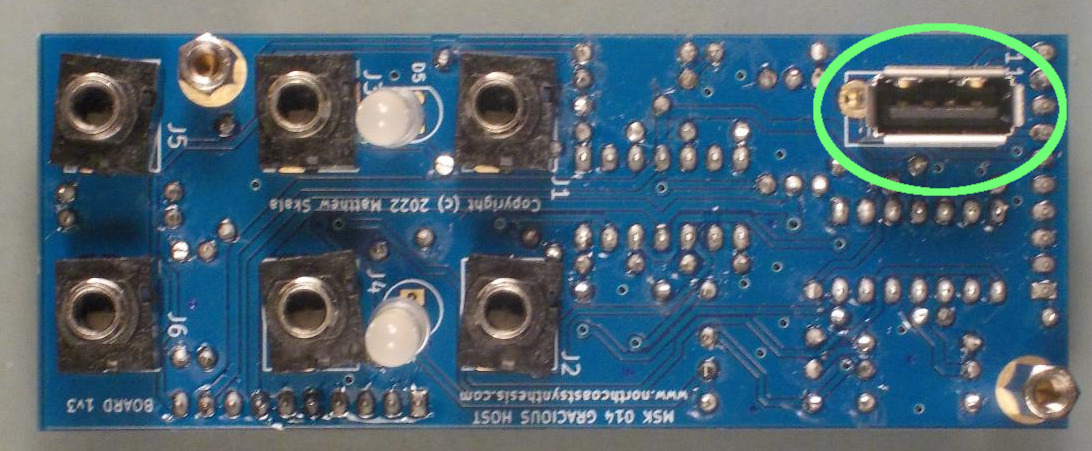
\includegraphics[width=\linewidth]{usb-a.jpg}

Line up the panel on top of the asembly.  Be sure that the top of the USB
connector fits into the panel hole provided for it and is not trapped under
the panel.  Fasten the panel in place by driving
the two machine screws through their corresponding holes into the 13mm
standoffs.

Carefully flip the assembly over and let the jack sockets fall into their
panel holes; the bushings should go all the way through the panel, with the
legs just poking through the circuit board.  Install the knurled nuts
provided for the jack sockets, to hold them in place on the panel.

Do not overtighten any of this hardware, and be careful, if you are
using wrenches or pliers, to avoid scratching the panel.  Wrapping the tool
jaws with tape may help.

Make sure that the LEDs poke through their corresponding panel holes by the
amount you prefer.  It may be necessary to push or pull on their legs at the
back of the board in order to get the depth right.

Solder all the panel components you just installed.

\section{Final assembly}

Insert the LM224 chips in their sockets on Board~1.  Be careful to insert
them right way round, with the Pin~1 markings on the chips matching those on
the board, pointing down toward the bottom of the finished module.

It should not be necessary to remove the panel from Board~1 again.  Just
attach Board~2, carefully fitting its header
plugs into the header sockets on Board~1 and the male ends of the standoffs
through the corresponding holes in Board~2.  Then use the hex nuts to fasten
Board~2 in place.

Install the configuration jumpers on J9, on Board~2.  Their function is
described in the ``general notes'' chapter of this manual.  The recommended
default configuration is to place jumpers in the locations marked G, C, and
5, which are the three locations at left, marked by a heavy line on the
board silkscreen.

\nopagebreak\noindent
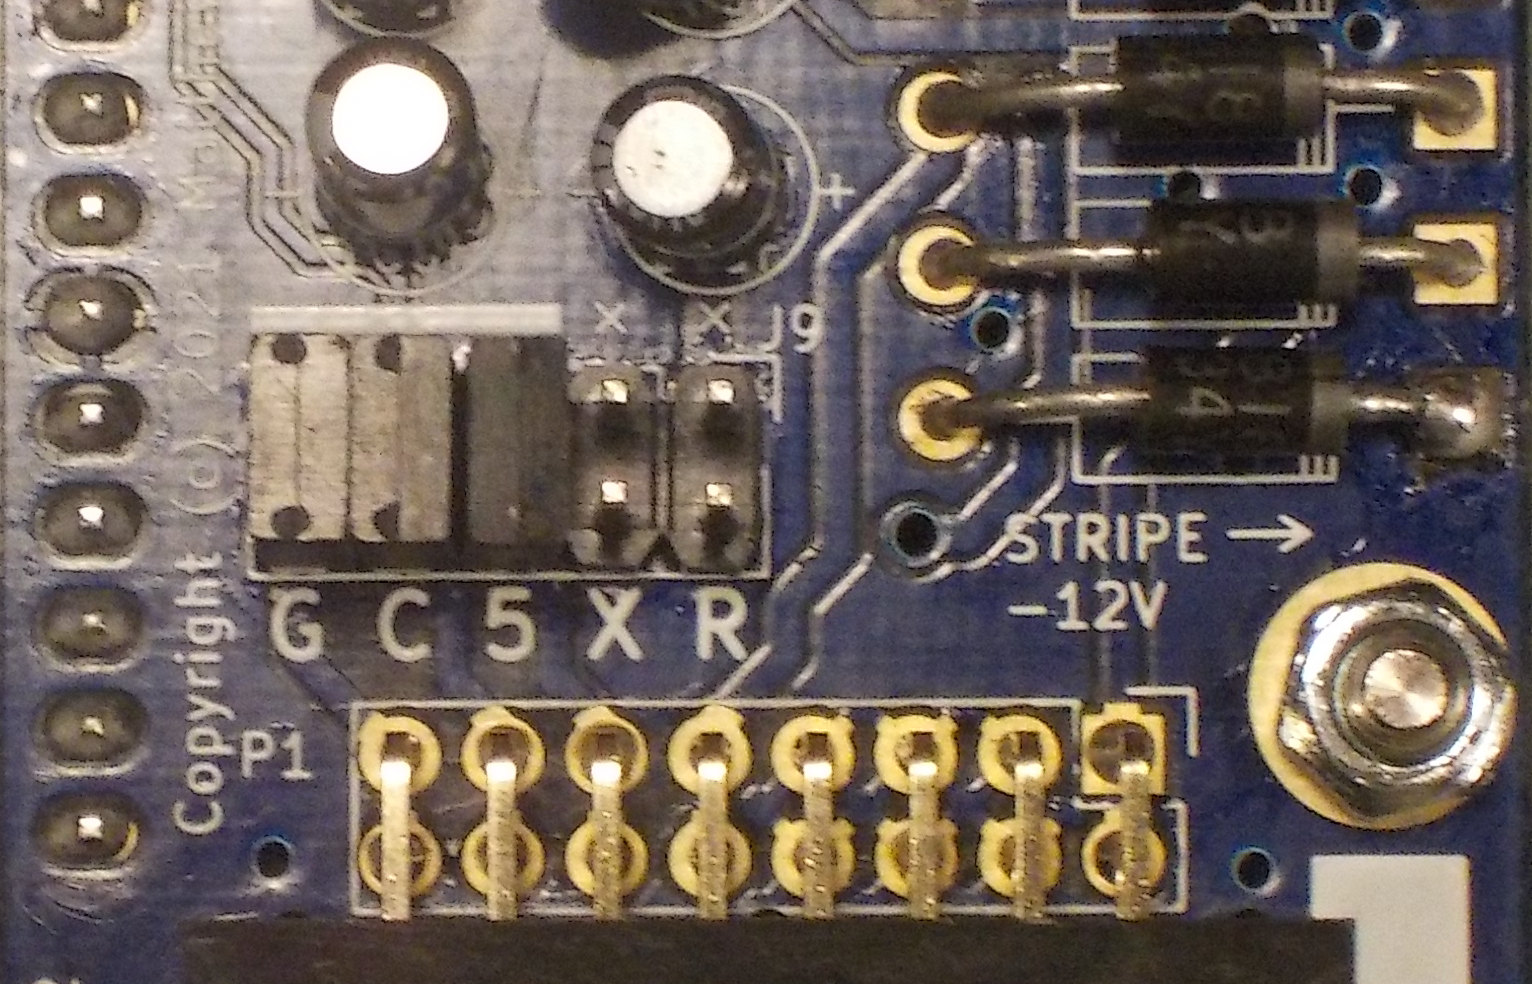
\includegraphics[width=\linewidth]{jumpers.jpg}

There is a rectangular white area at the right of Board~2 reserved for adding
a serial number, signature, quality control marking, or similar.  Use a
fine-tipped permanent marker to write whatever you want there.  Isopropyl
alcohol will probably dissolve marker ink, so do this step after any
board-cleaning.

The hardware of your module is complete at this point; but to get the
voltages as accurate as possible, you may wish to run the calibration
procedure described in the next chapter.

\nopagebreak
\noindent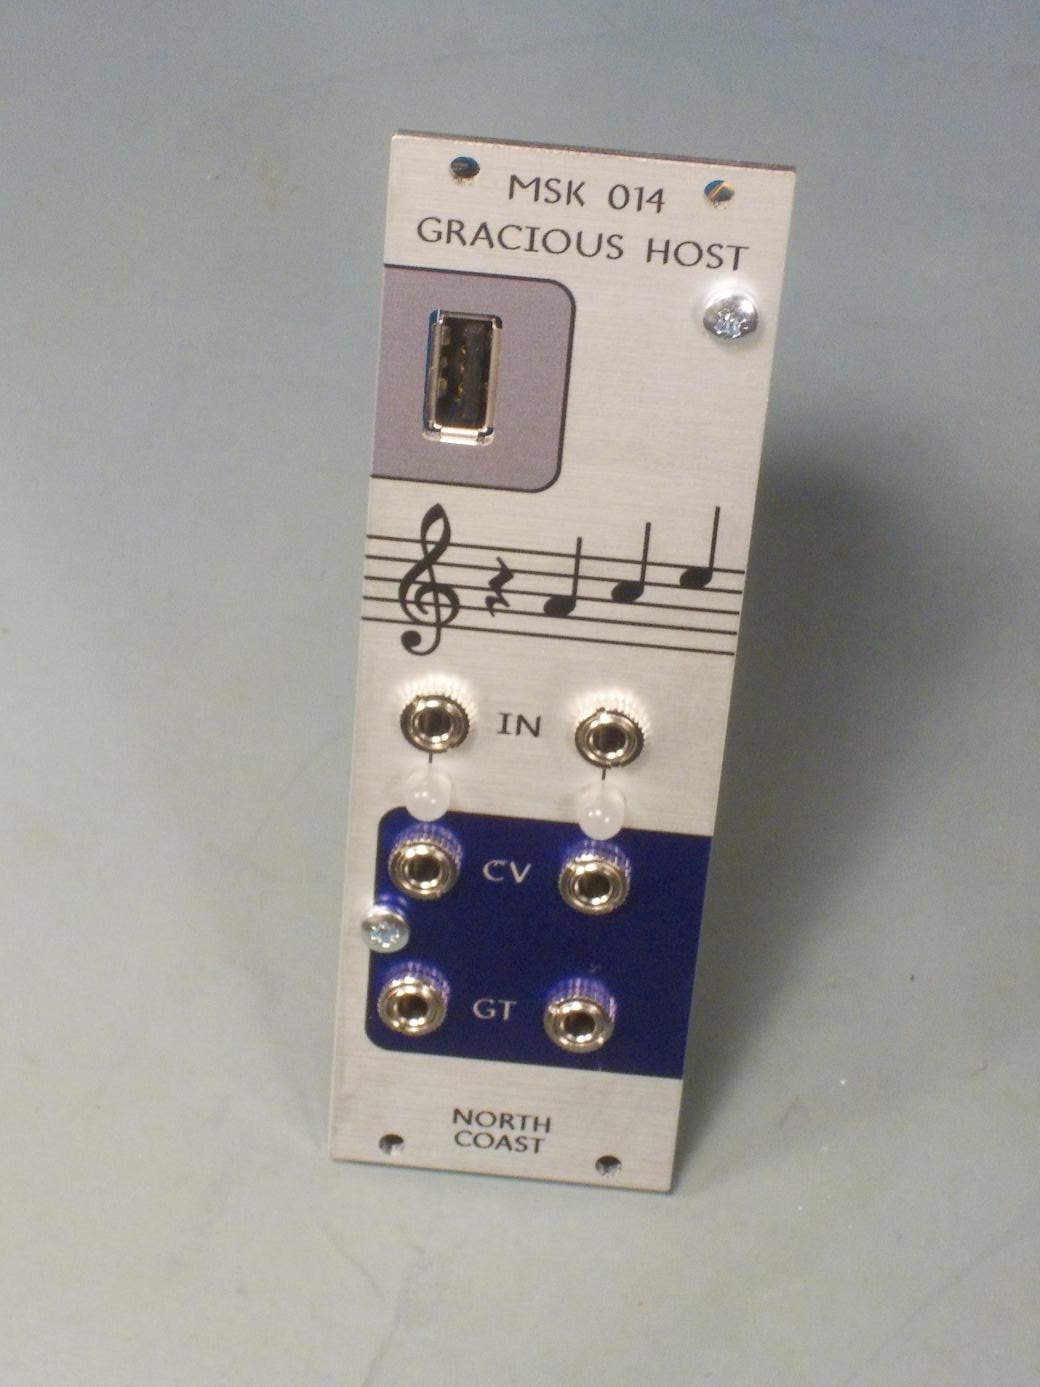
\includegraphics[width=\linewidth]{finished.jpg}
